
\section{Introduction}

By a curious coincidence, the typical escape velocity of massive galaxies is
such that $v_{\rm esc}^2/c^2$ is comparable to the apparent sizes of a
galaxies at cosmological distances.  This coincidence is fortunate,
because it makes the lensing deflection angle (which is $2v_{\rm
  esc}^2/c^2$) of distant galaxies comparable to their size on the
sky, and as a result, strong lensing by galaxies tends to produce
images that probe the dark halos of those galaxies.  This is
important, because while there is a general consensus that basic
mechanism of galaxy formation involves gravitational collapse,
fragmentation, and mergers of dark-matter clumps, into which gas fell,
cooling through radiative processes to form dense clouds and
eventually stars, there is much debate about the details \citep[for a
  summary, see][]{2012RAA....12..917S}.  In particular, the nature of
dark matter remains mysterious: most researchers take it to be a
collisionless non-relativistic fluid (cold dark matter or CDM) readily
studied by simulations \citep[for example, the influential millenium
  simulation by][]{2005Natur.435..629S}.  But other scenarios, where
dark matter has exotic dynamical properties
\citep{2010MNRAS.405...77S,2016ApJ...818...89S}, or is not really
matter at all but a modification of gravity
\citep{2016PhRvL.117t1101M}, have also been considered.

All this motivates using galaxy lenses to study the mutual dynamics of
dark matter, gas and stars in galaxies.  Several studies in recent
years have done so
\citep{2009ApJ...703L..51K,2011ApJ...740...97L,2012MNRAS.424..104L,
  2016MNRAS.459.3677L,2016MNRAS.456..870B} but it is desirable to
enlarge the samples from tens of lensing galaxies to thousands.  Doing
so requires both finding more lenses and also modelling their masses.
Recent searches through the CFHTLS \citep{2012SPIE.8448E..0MC} using
arc-finders
\citep[e.g.,][]{2012ApJ...749...38M,2014A&A...567A.111M,2014ApJ...785..144G,2017arXiv170401585S}
by machine learning
\citep[e.g.,][]{2016A&A...592A..75P,2017arXiv170302642L} and by visual
inspection by citizen-science volunteers in Space~Warps
\citep{2016MNRAS.455.1191M} have, between them, discovered an average
of four lenses per square degree, so one can be optimistic about
finding many thousands of lenses in the next generation of wide-field
surveys, from the LSST in optical and the SKA in radio on the ground,
and Euclid and WFIRST in orbit.

The expected flood of new lens discoveries will need a similarly huge
modelling effort to reconstruct their mass distributions.  To prepare
for the challenge of massive-sample lens modelling,
\cite{2015MNRAS.447.2170K} developed a new modelling strategy,
implemented as the SpaghettiLens system.  The idea is to collaborate
with experienced members of the citizen-science community, who have
already participated in lens discovery through \SW, as well as several
other projects involving astronomical data.  The system was tested on
a sample of simulated lenses, which were part of the training and
testing set in \SW.

This paper continues that study by applying SpaghettiLens to
lens-candidates discovered through Space~Warps.  We present results
from modelling of 58 of the 59 lens candidates reported by
\cite{2016MNRAS.455.1191M}.  Each lens candidate was modelled in a
collaborative refinement process, where anyone interested can create a
new model or modify an existing model to try and make it
better.\footnote{This is in contrast to the main Space~Warps project
  for discovering lenses, where volunteers in a crowd of $\gtrsim10^4$
  make independent contributions.  Each person is presented with a
  random selection of survey-patches and invited to (in effect) vote
  on each.  The system estimates each volunteer's skill level
  according to test-patches interspersed with the real data, and
  weights their votes accordingly \citep{2016MNRAS.455.1171M}.  There
  is an active forum for volunteers, but since everyone is seeing
  different data samples with minimal overlap, the forum has little if
  any influence on votes.}  The resulting model represents a consensus
among contributors, as to the best that could be achieved with the
available data and software.

Interpretation of the results is tentative,
because the systems are lens candidates at this stage, not secure lenses.
Moreover the candidate-lens redshifts have large uncertainties, while
the candidate-source redshifts can only be guessed at present.
Nevertheless it is interesting to see what trends we can observe with
the already-available data.
%TODO there is more info about uncertainies here:
% https://arxiv.org/pdf/0811.3326.pdf

This paper is organized as follows:
Section~\ref{sec:candidates_models} introduces the candidates, the models and the diagnostics applied to them.
The following sections elaborate on the diagnostics.
Image morphology diagnostics are explained in Section~\ref{sec:morph} and
diagnostics based on the mass models in Section~\ref{sec:massmodels}.
Stellar masses are calculated in Section~\ref{sec:stellar-mass} to compare stellar to lensing masses of the lensing candidates.
Section~\ref{sec:summary} gives our summary and conclusions.

There are three appendices devoted to various technical issues
relating to modelling.  \cite{2015MNRAS.447.2170K} tested the system
on simulated lenses and identified some areas for improvement.  In
\S~\ref{subsec:sourcefit} we introduce fitting of the brightness
profiles of the source.  This feature has not yet been included in
SpaghettiLens, but has been carried out in post-processing for a few
especially interesting candidates.  In \S~\ref{subsec:hires} we show
that making mass maps fine-grained in the central region relieves a
tendency in the earlier work for mass profile to be too shallow. Then in
\S~\ref{subsec:parameter} we consider the possibility of fitting a
parametric lens model to the model ensemble; so far we have only been
successful at extracting an Einstein radius.

The online supplement gives results for all the modelled systems generated
for all the lensing candidates.




\section{The candidates and models}
\label{sec:candidates_models}

\SW is a citizen science gravitational lens search \citep{2016MNRAS.455.1171M}.
Its first run searched the CFHT Legacy Survey, a survey carried out in five optical bands ($u^*$,$g'$,$r'$,$i'$,$z'$) covering a total area of 160 \sqdeg, divided up into four fields.
It has a field of view of 1 \sqdeg, a pixel size of 0.186'' and the deepest limiting magnitude is 25.47 in the $g$ band\citep{2012AJ....143...38G}.
The cutouts shown to the volunteers were colour composites of the $g$, $r$ and $i$ band of randomly chosen regions.
It resulted in 59 new (of which 29 promising) lens candidates that have not been found by other searches already and in the rediscovery of 82 previously known lens candidates.
The candidates have broadly similar redshifts (0.2 -- 1.0), Einstein radii (0.7\arcsec -- 5\arcsec) and arc magnitudes (22 -- 26) as previous robotic robotic searches by ArcFinder and RingFinder \citep{2016MNRAS.455.1191M}.

\begin{figure}
  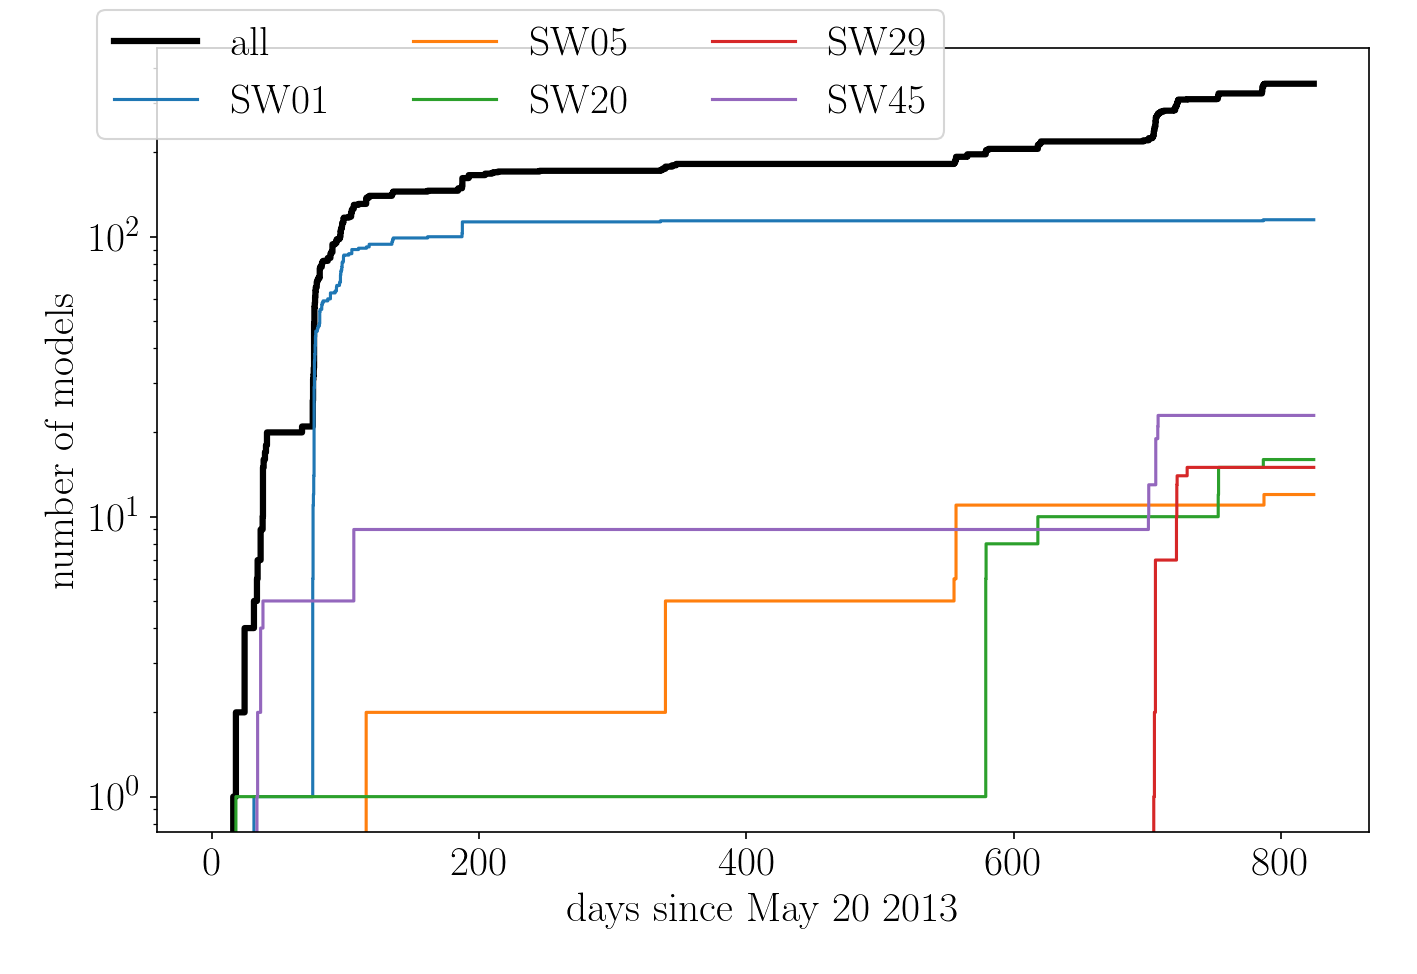
\includegraphics[width=\linewidth]{img/timelapse3}
  \caption{ Number of models generated over time in days since an arbitrary starting point; black line shows all models, colored lines show five most active candidates. Total of 365 models were generated for 56 lens candidates, eight users contributed more than five models per person. }
  \label{fig:time}
\end{figure}

While \SW was running, volunteers started working with \SpL to create models of possible lensing candidates found in \SW that were debated on the \SW discussion forums, before they were classified as plausible candidates.
Figure~\ref{fig:time} shows the total number of models generated over time, models created for systems that turned out to be non candidates were not included.
The first beta version of \SpL was launched in May 2013 and additional features were implemented on the fly.
The system was tested by eight major contributors, volunteers that at least generated five models.
In the beginning of August 2013 (day 70) a modelling challenge for the candidate later to be identified as \sw{01} was launched.
A group of five volunteers converged to a set of favourite models that they presented in an online letter after about 65 days and 30 models have been created for this particular system.
In April 2015 (day 700) the first full version of \SpL was presented for testing.
In the same time the list of identified candidates was made available \citep[as a preprint of the later work][]{2016MNRAS.455.1191M}.
At this stage, the volunteers were asked to complete the sample and to create models for all the lens candidates that were still missing.
The generated models for candidate \sw{29} show that the volunteers converged to a favorable model much faster, after 15 models generated in 30 days.
This modelling effort resulted in a set of 356 \SpL models for all but one of the \SW 59 lens candidates; candidate \sw{39} was not modelled.


We characterise each model with seven diagnostics, grouped into three 
categories, whose purpose is to help identify which systems are most probably 
lenses, and which ones are likely to be most rewarding for future follow-up 
observations. The diagnostics are as follows.

\begin{itemize}
\item First we have diagnostics based on morphology of the
  system.
  Section~\ref{sec:morph} and Figure~\ref{fig:splinput} explain.
\begin{enumerate}
\item Whether the images are unblended.  Distinct unblended images are
  an advantage in modelling, but not essential.
\item Whether all images are discernible.  The topography of an
  arrival-time surface, as encoded by a spaghetti diagram, may require
  more images than are visible, in which case the modeller has to
  insert conjectural image positions.
\item Whether the lens is fairly isolated.
\item The image morphology concisely described: double or quads,
  further sub-categorised to indicate the elongation direction of the
  lensing mass.
\end{enumerate}
\item Second we have mass models, covered in Section~\ref{sec:massmodels}.
\begin{enumerate}
\setcounter{enumi}{4}
\item Whether the mass map is reasonable. Figure~\ref{fig:kappa}.
\item Whether the arrival-time surface and synthetic image are
  plausible.  In particular, additional images are implied in regions
  where they are not observed signal an unsatisfactory model.
  Figures~\ref{fig:arriv} and \ref{fig:synth} and \ref{fig:encl}.
\end{enumerate}
\item Third, whether the total implied lensing mass
  determined from the lens model is plausible, given the
  photometry of the lensing galaxy.
  In this work we define lensing mass as the sum of all mass tiles
  needed to model a lens. These mass tiles reach out to typically twice
  the radius of the the outermost image.
  Section~\ref{sec:stellar-mass}
  explains how we compare the lensing mass with the mass in stars in
  the lensing galaxy.  We estimate the stellar mass by comparing
  galaxy magnitudes from the CFHTLS pipeline with the well-known
  stellar-population models of \cite{2003MNRAS.344.1000B}.  We then
  extrapolate the stellar mass to a halo mass using the
  abundance-matching prescription of \cite{2010ApJ...710..903M}.
  Naturally, the lensing mass must be more than the stellar mass but
  no more than the total halo mass.
\begin{enumerate}
\setcounter{enumi}{6}
\item We then introduce what we call a halo index ($\haloindex$) which
  gives an idea of how the lensing mass compares with these two
  constraints.  Figure~\ref{fig:stelmass}.
\end{enumerate}
\end{itemize}

Section~\ref{sec:summary} summarises and tabulates the diagnostics in
Table~\ref{tab:models}.




